\section{Multitouch Table}
The multitouch table created for the project is a rear diffused illumination design (see figure \ref{fig:mtdiagram}), and is housed in a core‐ten steel cabinet with recessed cooling fans and an access panel on the rear vertical wall.  The touch surface is a 1⁄2" polycarbonate sheet with an adhesive projection film applied to the underside (acting as a diffuser for the projected image).  

In addition, infrared light is also projected at the diffuser from below (inside the cabinet) the touch surface. The table currently uses an array of six multiple IR LED lamps. When an object touches the surface it reflects more light than the diffuser or objects far away from the surface. The change in light is detected by a web cam placed inside the cabinet, and the signal is fed to the computer for analysis.

\begin{figure}[htp]\centering
  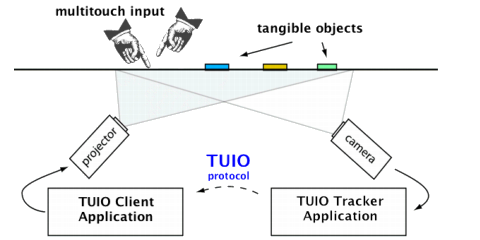
\includegraphics[width=.8\textwidth]{images/mt-diagram.png}
  \caption{This diagram explains the flow of information from a finger press to the reaction on the screen. \cite{REACT}}\label{fig:mtdiagram}
\end{figure}
\subsection{Software}
The multitouch table uses The Beta, from the NUI Group \cite{NUI}, to process the video stream from the webcam. The Beta, tbeta for short, is an open source tool that analyzes a video to find tracking data for objects it recognizes as fingers or cursor devices. The software provides a great deal of control over the video parameters (high-pass filter, amplification, threshold, etc.) that adapts well to many types of multitouch displays.

Tbeta outputs the tracking data using the TUIO protocol \cite{TUIO}, which is an open framework for receiving input events in various programming environments. For this project, the TUIO events sent by tbeta were received using the open source Java TUIO library in a Processing sketch. 
